現代で通信という言葉を聞いた時、連想される多くはインターネットを始めとした様々な電気通信だろう。だが、電気通信ができる以前より、人は様々な意思疎通…通信を行ってきた。本章では、電気通信に至るまでの人の意思疎通の営みを見ていく。これらの営みの中で、人間は通信に必要とされる要件を見出してきた。通信とは何か、何が必要なのか。まずは歴史からその要件を学び取っていこう。

\section{声による伝達}

動物には種によって様々な対話方法がある。蝙蝠なら超音波を使い、鳥ならば鳴き声で対話を行う。動物の鳴き声のモノマネで知られる江戸家小猫氏によれば、人間に最も近いゴリラなどは10種類の鳴き声により様々な対話を行うという。例えば、我々がゴリラの鳴き声と聞く「ウホウホ」という鳴き声は、特に喜ばしい時、幼いゴリラが使うことが多い表現なのだそうだ。我々人間にその差異はなかなかわかりづらいが、しかしながら種ごとの鳴き声による伝達は、我々人間の発話による伝達に同じことなのだという。

\subsection{人間の発話}

自らの声帯により何らかの音を出し、これに意味を持たせて伝達する。我々人間が知る多くの動物の鳴き声にはそれほど多くの種類の伝達はなく、概ね自らの感情の伝達が中心となっているようではあるが、人間の発話による伝達もそれと同様である。生まれてすぐの赤子は、泣くという動作を伴った発話により自身が不快であることを伝える。成長し、感情が分化する(図\ref{fig0_1})につれ、何が不快なのかなどもその泣き方に入ってくるようで、親はその泣き方で状況を察することも少なくない。やがて、言葉を覚え話すようになると、それらの言葉の意味を経験から学ぶようになる。家族から広がるコミュニティの中で、共通した意味の言葉を使うようになり、人との伝達・コミュニケーションを始めていくのである。

\begin{figure}[htbp]
\centering
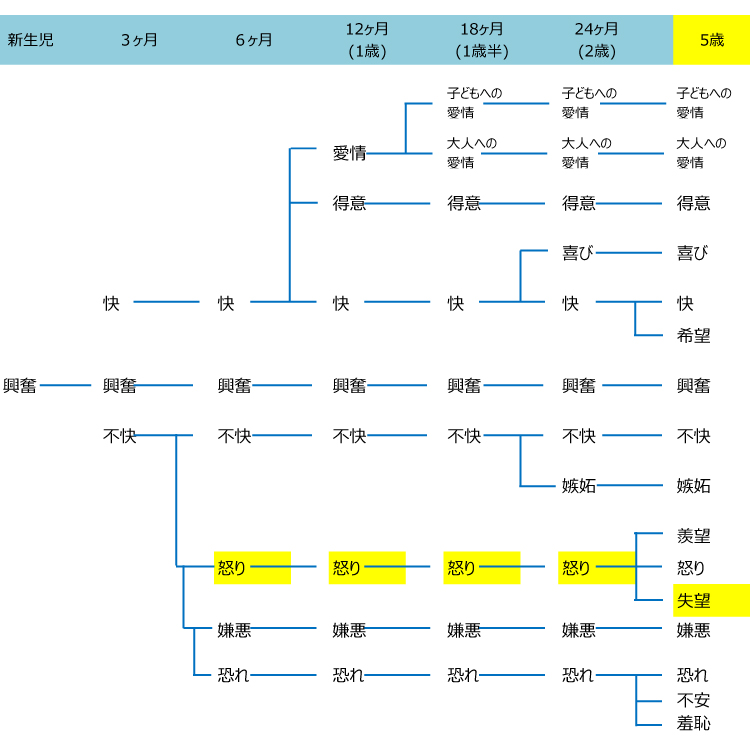
\includegraphics[width=0.6\linewidth,keepaspectratio,bb=0 0 750 750]{fig/fig0_1.jpg}
\caption{ブリッジスの情緒分化図 日本病児保育学会ブログ記事より引用}\label{fig0_1}
\end{figure}

コミュニティの違いによる差異こそあるものの、我々人間の"鳴き声"は言語を為し、その共通認識により対話、伝達が始まったのである。この言語は感情にとどまらず、具象抽象の垣根を超えて叙事や論証、または歌や言葉遊びと言った様々な知的活動の礎となった。動物の鳴き声による対話と対応した人間の会話は、最も原始的な伝達の方法であるものの、様々に技術が発達した今なおコミュニケーションの基礎を為している。通信の始まりは、このような"発話による伝達"であったといえよう。

\subsection{発話の制約}
しかし、単純な発声による発話では、声が届く範囲にしかその意味が届かない。この時の届く範囲とは、空間的な範囲もあれば時間的な範囲でもある。落語会が行われていた会場に、終わった後に入っても落語を聞くことはできないし、また、同じ時間に遠く離れた場所にいても落語を聞くことはできない。肉声の落語を聞くことができるのは、その時その場所で演者と同じ空気を共有していた者に限られる。逆に、その空気を共有している者の中では、選択的に伝えたり聞いたりするということも難しい。高座の上で演者が下座に何らかの指示を出す時、声を使うとすれば客席の幾人かにはどうしても聞こえてしまう。同じ会場で鼾をかいて眠る客がいたとして、これだけを聞かないというのもなかなか無理がある。

先の鼾の例のような雑音があった場合などは特にそうだが、発話によるコミュニケーションでは聞き取れない・追いつかないと言った問題も発生する。マンツーマンのゆっくりした対話であれば言い直してもらえばすむだけの話であるが、先の落語のような例では、そういうわけにも行かない。音自体が聞こえなかった、音は聞こえたけれども判別がつかなかったと言ったレベルから、言語的な問題…イントネーションの差異、語彙にない単語の使用、そもそも言語が異なる、勘違い…と言った知識や思考の問題まで、発話の時には伝達の誤りが起こりうる。

発話による伝達は、原始的であるがゆえに手軽ではあれど制約や問題も内包している。通信・伝達技術というのは、これらの制約や問題を如何に打破するのかという人間の飽くなき挑戦の成果であるとも言える。

\subsection{口伝という方法}
発話の制約を最も単純に外したのは\textbf{口伝}\index{くでん@口伝}である。現在でも民話や民謡など、様々なものが口伝により伝えられているが、これは人間の記憶を介することによって時間や空間の制約を緩和したものといえよう。最も身近なところでは、伝言がそうであろう。もっとも、伝言ゲームに見られる通り、伝達の誤りという問題は解決されているとは言いがたい。「JPCZによる擾乱の影響で山陰地方を中心に荒天となる」などと専門の用語が入った言を伝言したところで、途中に知らぬ人が入れば伝言がうまく行く可能性は低いだろう。また、伝言には意識的・無意識的な取捨選択もあり、伝達の誤りという観点ではむしろ増えているかもしれない。

しかしながら、人間以外の資源が必要ないこの口伝という方法は、最も初期から存在すると同時に、現代まで続いている伝達方法である。口伝の国内における最も古い例としては、稗田阿礼が挙げられる。古事記には彼(彼女?)の誦により伝えられたものが筆録されている。その後の歴史にも、説法や講釈と言った例はほぼ口伝であったようだ。一方、現代で行われている口伝の例としては、先にも持ちだした落語を例に挙げたい。昭和の爆笑王、桂枝雀師は著書「枝雀とヨメはんと七人の弟子」の中で次のように書いておられる。

"一番最初は「ちょっとやるから聞いてなさい」と言って、一字一句口移しで教えることから出発いたします。やらせてみて、ちょっと違うとイントネーションから直す。それが段々お稽古やっていくうちに、五分なら五分、流れを教えるようになる。"

これは、平成のはじめ頃に書かれた文であるし、枝雀師は99年にお隠れになったから、いま他の噺家が同様のやり方をしていると言い切ることはできない。だが、筆者が、この枝雀師の三番弟子、文之助師に"つる"を教わった時は、ほとんどこの通りの教え方であった。ただ、カルチャースクールでのことであるから、録音し、自分で原稿に起こし、その上で直してもらいながらという指導であった。とはいえ、これも口伝には違いない。多くの伝達法がある中で、わざわざこの原始的な口伝という方法で伝承をするのはなぜだろうか。

それは、口伝によってしか伝えられない、空気や情感、発生、身振り手振りの細かな違いなどを伝えられるというところであろう。現代の技術をもってすれば、双方向で似たような指導を遠隔地間で行うことも可能であるように見える。しかし、それでも微妙な空気感や息の間といったものは伝えきれない。落語という芸能は高座の落語家と客席が一体となって作り上げる空間が生命であるから、なるほど、その部分を伝えるためには口伝を取るよりほかないのであろう。また、落語は時代により変化していくものであるから、口伝という形態での変化は逆に追い風となるのであろう。これは、落語の伝承が「ネタの原稿を伝える」のみでないことを示しているといえる。

現代の視点からすれば口伝は古臭く、非効率な手法に見えることも多い。だが、それを意図して取り込んでいる芸に学べる通り、口伝でこそ伝わることもある。通信・伝達技術の多くは、重要と考えにくいものや伝えづらいものを取捨選択しているのである。逆に、その捨てられたものを拾う価値があるシーンや、そこまでの効率を要求しないシーンがあるからこそ、一見古臭く見える通信・伝達の方法も現代に息づいているのである。

\section{書くことによる記録}

口伝は人間の記憶を媒介にして時間や空間の制約を打ち破った。しかしながら、当然全ての人間が稗田阿礼のような記憶力を持つはずもないし、伝達も記憶も個人の状況に依存することとなる。これを打破するのは日本へと輸入された文字であった。

文字とそれを記録する媒体は、ヒエログリフやパピルスと言った著名な例があるとおり古代エジプト文明の時代にまで遡る。楔形文字や漢字と言った様々な文字が青銅器時代に生まれたのである。日本へ文字が入ってくるのは弥生時代とされ、それからの後、8世紀頃には先の稗田阿礼の言を元にした古事記(図\ref{fig0_2})や風土記、日本書紀と言った書物が発行された。

\begin{figure}[htbp]
\centering
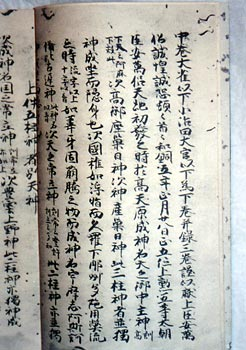
\includegraphics[width=0.6\linewidth,keepaspectratio,bb=0 0 246 350]{fig/fig0_2.jpg}
\caption{真福寺収蔵の国宝・『古事記』 Wikipediaより引用}\label{fig0_2}
\end{figure}

文字の輸入に伴い、離れた場所に文字を書いた媒体を送るという形式での伝送も行われるようになっていった。それらの書物の中には何百年という時を経てなお現代で読むことができるものも多い。これは、文字とその記録媒体が時間と空間の制約を打ち破ったということである。著名な数学者の書簡や日記が見つかることもあれば、伝わるつもり無く詠まれた"この世をば 我が世とぞ思う 望月の 欠けたることも なしと思えば"が現代にまで伝わっている(道長本人は記録に残さなかったが、その場に居合わせた人が日記に記したために現代まで伝わっている)など、文字は言語によって表現可能なものの時間的・空間的制約を打ち破ったのである。汚損や焼失といったリスクこそあるものの、口伝や発話の段階からすれば大きく進歩したと言えるのは明らかであろう。

また、これらの媒体は図画の伝達も可能とした。これは、発話や口伝で伝えられなかったものを伝えられるという利点をもたらした。紙媒体は、文字を媒介に発話を記録すると共に、図画として描けるものも記録する媒体なのである。

\subsection{複写}
書物として残されていく

\subsection{紙媒体が捨てたもの}


\section{遠距離の高速通信:狼煙・手旗信号}


しかし郵便は時間がかかります。ではもっと早く伝えたい場合はどうすればいいかというと、視覚に訴えるものを使えばいいという考えに至りました。

このときに「では煙で通信しよう」となって開発されたのが狼煙です。
また、見える範囲ならば情報をリアルタイムに伝えられる通信として手旗信号といったものも開発されました。

このように口伝から書簡や狼煙、手旗信号に通信の手法を変えることで、遠くに素早く通信できたり、時を越えて通信することができるようになりましたが、言葉にこめられる口調や声の違いといった情報を代わりに失いました。

\section{公開と複製:模写・印刷}

人間は書簡といった文字を記録する媒体を使ううちに、その情報をたくさんの人々に公開するために複製しようと試みるようになりました。

最初は紙に書き写すといった作業だけであったのが、版画で同時に並行して複製ができるようになり、コピー印刷で膨大な量の複製が可能になったりと、時代を重ねるごとに複製の量と質が格段に向上していきました。

\section{通信の秘匿:シーザー暗号・方言での暗号}

ここまでは「広める」通信について考えてきましたが、やはりどうしても人には秘密にしたいことを特定の人に伝えたい場合というときはあるものです。
しかし戦場ではまだ書簡を使って通信していましたが、奪われてしまうといったリスクはどうしても拭いきれませんでした。
このときに情報の秘匿性を高めるために暗号が開発されました。

代表的なものだとシーザー暗号が挙げられます(内容は下記の練習問題を参照)。このような一対一で文字変換を行う暗号を単一換字式暗号と言います。

一方で第二次世界大戦中は薩摩弁が難解であるため暗号として使われたのですが、敵軍の日本人捕虜に傍受した暗号を読ませて平文に変換してしまっていたそうです。
このように暗号としてほとんど意味を成さなかったものも存在します。


\section{記録媒体の変化と増加}

記録媒体というものは時代とともに変化していきます。

ここまでの例だと最初は紙や石版などに文字を書き込むというところから始まり、版画やコピーへと移り変わっていったというようなものです。実際このような移り変わりの中で、記録媒体の数は増加していきました。

では現在使われている記録媒体は昔のどんなものからきたのでしょうか。

\subsection{活動写真という媒体}

活動写真は今の映像の記録媒体の発展に深く関わっている媒体です。
概要としては、観客を呼んで動画を見ながら横で活動弁士と呼ばれる人がその映像について解説する、といったものです。

この活動弁士の音声と活動写真の映像を一緒にしてしまおうと作られたのが映画で、それを映画館などではなく一人で見たいという人のために映画を記録する媒体がビデオテープ、DVD、BDとして開発されました。

このように、活動写真は今の映像記録媒体の発展に大きく役立った存在であると言えます。

\section*{演習問題}
\begin{problems}
\item 歴史的なシーザー暗号では、アルファベットを3文字後ろにずらして(a,d,x,y,zをそれぞれd,g,a,b,cに変えるなど)暗号化していた。1024文字以下1行の半角文字列が入力されるとき、それをシーザー暗号化・復号化するプログラムを作成せよ。
\end{problems}
